\section{Application Acceleration}
\subsection{Hardware-Accelerated Grep}

\subsection{Linear Algebra Operations}

Vector/Vector multiplication

Two vectors are both stored on the distributed flash.
Multiplication is done by telling the fpgas the pages where the data is
stored. This is a good example because the resulting value is just a single
value.

Sparse Matrix addition?
Sparse Matrix Mult?

\begin{figure}[h]
	\begin{center}
	%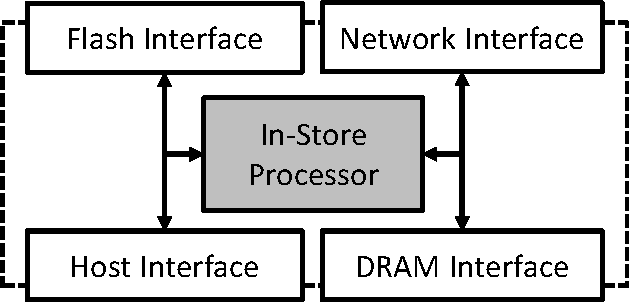
\includegraphics[width=0.3\paperwidth]{figures/isp-service-crop.pdf}
	\caption{Linear Algebra Acceleration Results}
	\label{fig:result_algebra}
	\end{center}
\end{figure}
